\documentclass{article}
\usepackage[utf8]{inputenc}
\usepackage{tikz}
\usepackage{xcolor}
\usepackage{geometry}
\usepackage{amssymb}

% Page setup to mimic a slide
\geometry{a4paper, margin=1in, top=0.5in}

% Define colors to match the source image
\definecolor{titleblue}{RGB}{0, 51, 102}    % Dark Navy for Title
\definecolor{headerblue}{RGB}{30, 144, 255} % Light Blue for Header border
\definecolor{userdatagreen}{RGB}{34, 139, 34} % Green for User Data borders

\usetikzlibrary{arrows.meta, positioning, bending}

\begin{document}
\pagestyle{empty}

% --- Header / Title Section ---
{\huge \textbf{\textcolor{titleblue}{FreePageFile}}} \\
\vspace{-5pt}
\hrule
\vspace{30pt}

% --- Diagram Section ---
\begin{center}
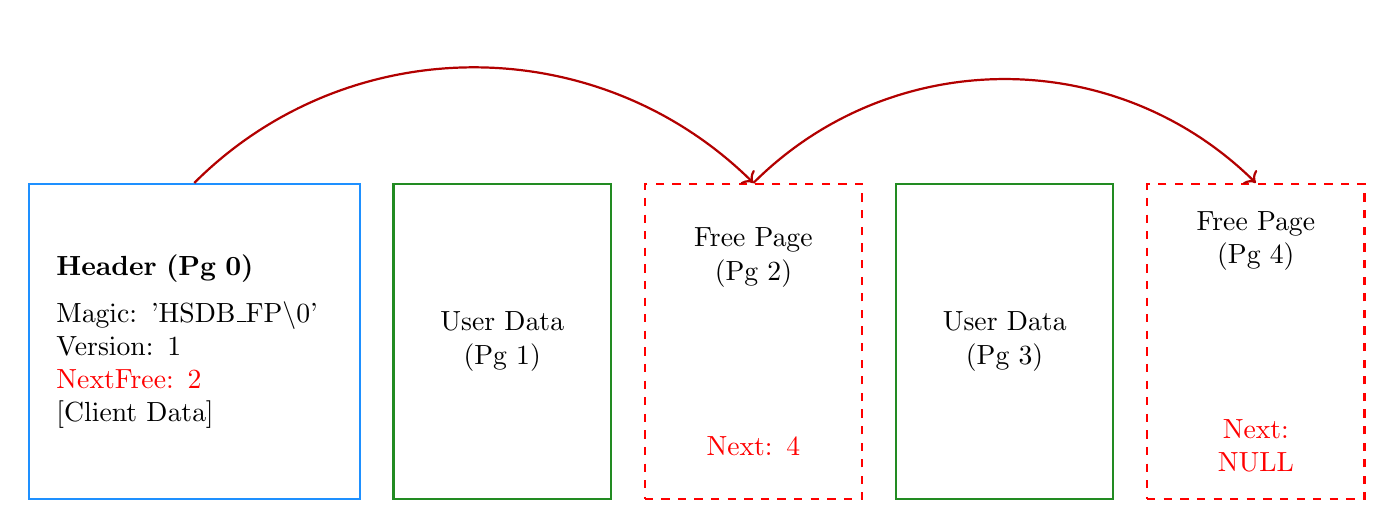
\begin{tikzpicture}[
    node distance=0.4cm,
    header_style/.style={draw=headerblue, thick, align=left, text width=3.5cm, minimum height=4cm, inner sep=10pt},
    user_data_style/.style={draw=userdatagreen, thick, align=center, text width=2.2cm, minimum height=4cm, inner sep=8pt},
    free_page_style/.style={draw=red, dashed, thick, align=center, text width=2.2cm, minimum height=4cm, inner sep=8pt}
]

% Node 0: Header
\node[header_style] (h) {
    \textbf{Header (Pg 0)} \\
    \vspace{5pt}
    Magic: 'HSDB\_FP\textbackslash 0' \\
    Version: 1 \\
    {\color{red}NextFree: 2} \\
    \vfill
    [Client Data]
};

% Node 1: User Data
\node[user_data_style, right=of h] (p1) {User Data\\(Pg 1)};

% Node 2: Free Page
\node[free_page_style, right=of p1] (p2) {Free Page\\(Pg 2)\\ \vspace{1.8cm} {\color{red}Next: 4}};

% Node 3: User Data
\node[user_data_style, right=of p2] (p3) {User Data\\(Pg 3)};

% Node 4: Free Page
\node[free_page_style, right=of p3] (p4) {Free Page\\(Pg 4)\\ \vspace{1.8cm} {\color{red}Next:\\NULL}};

% --- Curved Arrows ---
% Arrow from Header to Pg 2
\draw[->, thick, red!70!black, bend left=45] (h.north) to (p2.north);

% Arrow from Pg 2 to Pg 4
\draw[->, thick, red!70!black, bend left=45] (p2.north) to (p4.north);

\end{tikzpicture}
\end{center}

\vspace{30pt}

% --- Text Content Section ---
\begin{itemize}
    \setlength{\itemsep}{10pt}
    \item[] \textbf{Stores data in 4KiB pages}
    \begin{itemize}
        \item[] $\bullet$ Avoids external fragmentation, at the cost of internal fragmentation
        \item[] $\bullet$ = Sector size on modern SSDs
        \item[] $\bullet$ = Page size on modern OSs
    \end{itemize}
    
    \vspace{10pt}
    \item[] \textbf{allocatePage() and freePage()}
    
    \vspace{10pt}
    \item[] \textbf{Keeps free pages in a freelist}
    \begin{itemize}
        \item[] $\bullet$ Inserts (free) and deletions (allocate) in $O(1)$
    \end{itemize}
\end{itemize}

\vfill

% --- Footer ---
\hfill \footnotesize 11/30

\end{document}
